\documentclass{article}[12pt]
\usepackage{physics}
\usepackage{setspace}
\usepackage{amsmath}
\usepackage{mathrsfs}
\usepackage{amssymb}
\usepackage{feynmp-auto}
\usepackage{tgtermes}
\usepackage{graphicx}
\usepackage{booktabs}
\usepackage{array}
\usepackage{caption}
\usepackage{listings}
\usepackage{xcolor}
\usepackage{helvet}
\usepackage{float}
\definecolor{codegreen}{rgb}{0,0.6,0}
\definecolor{codegray}{rgb}{0.5,0.5,0.5}
\definecolor{codepurple}{rgb}{0.58,0,0.82}
\definecolor{backcolour}{rgb}{0.95,0.95,0.92}
\definecolor{lightgray}{rgb}{0.95,0.95,0.95}
\bibliography{Master_Thesis}
\lstdefinestyle{mystyle}{
    backgroundcolor=\color{lightgray},   
    commentstyle=\color{codegreen},
    keywordstyle=\color{magenta},
    numberstyle=\tiny\color{codegray},
    stringstyle=\color{codepurple},
    basicstyle=\fontfamily{pcr}\selectfont\footnotesize,
    breakatwhitespace=false,         
    breaklines=true,                 
    captionpos=b,                    
    keepspaces=true,                 
    numbers=left,                    
    numbersep=5pt,                  
    showspaces=false,                
    showstringspaces=false,
    showtabs=false,                  
    tabsize=2
}
\numberwithin{equation}{section}
\lstset{style=mystyle}
\captionsetup{font=footnotesize}
\newcommand{\RN}[1]{%s
  \textup{\uppercase\expandafter{\romannumeral#1}}%
}
\usepackage{geometry}
\geometry{
 a4paper,
 left=25.4mm,
 right=25.4mm,
 top=30mm,
 bottom=25.4mm
 }
\begin{document}
From the circuit in Figure 3, we can establish the circuit equation for the Josephson junction:

\subsection{LC circuit}

First, assume the following closed LC circuit:

\begin{figure}[htbp]
    \centerline{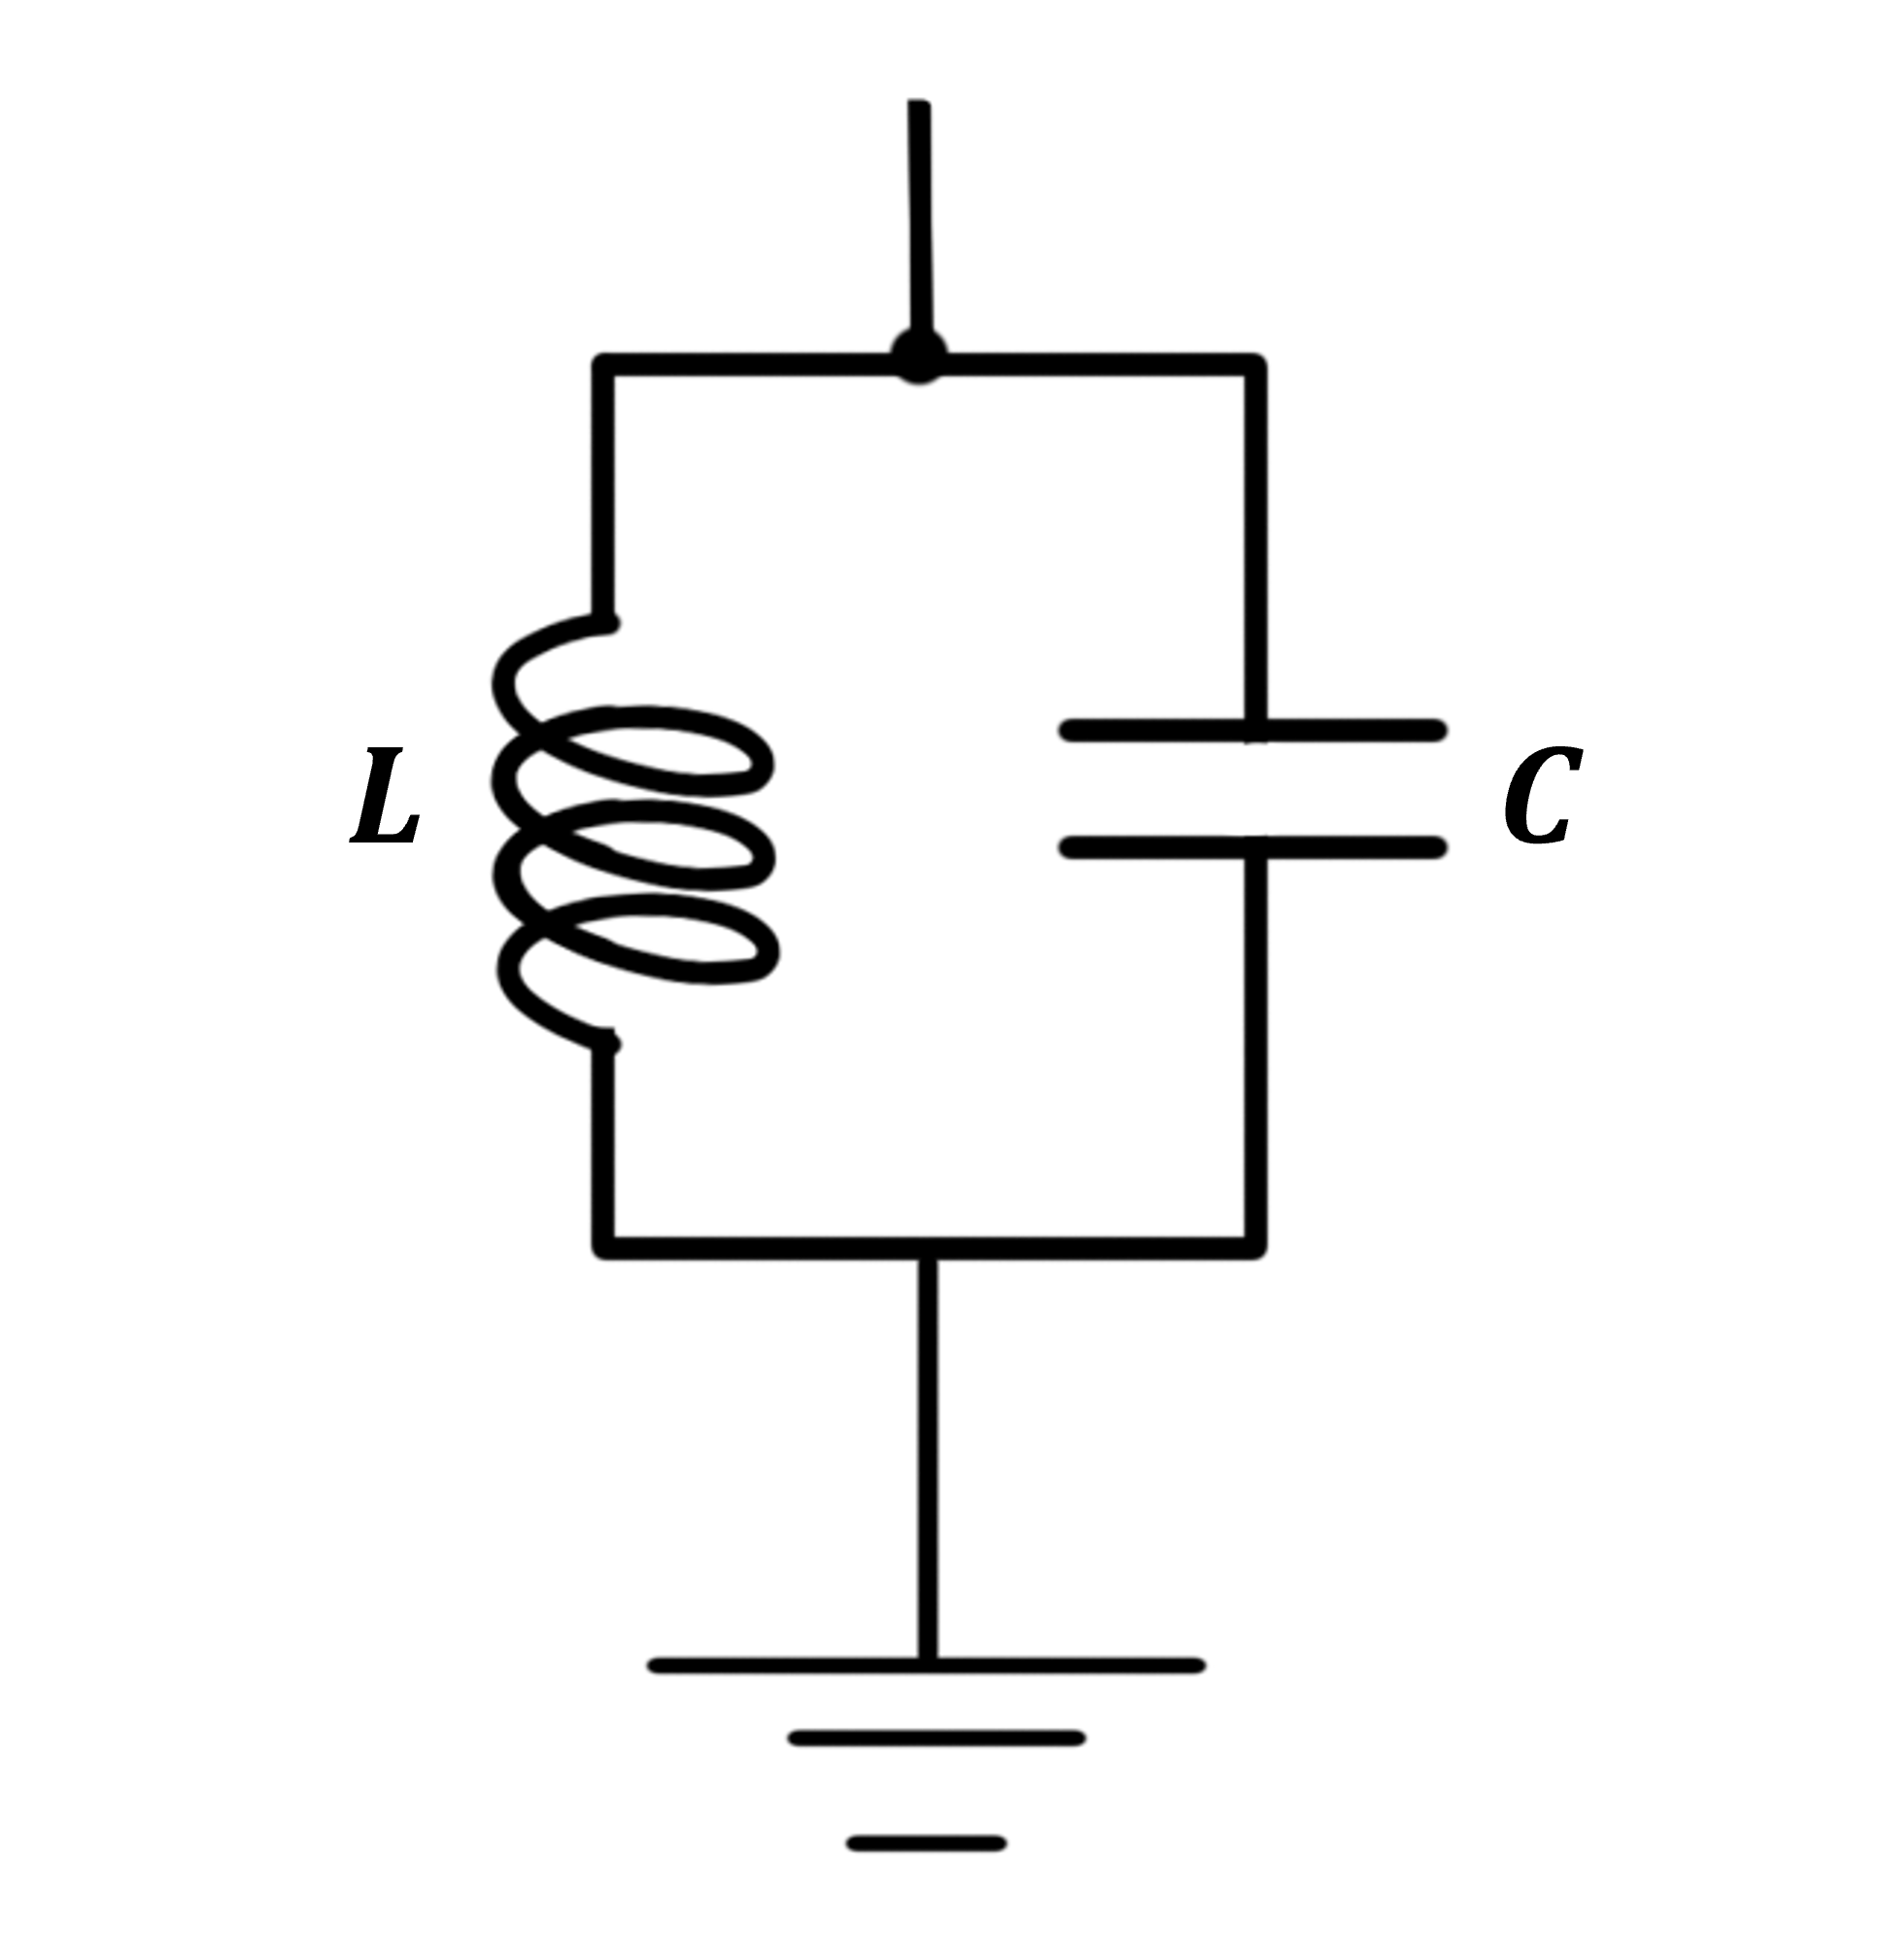
\includegraphics[width=5cm]{TexFigure/LCcircuit.png}}
    \caption{LC circuit in closed loop}
    \label{fig:reentrant}
  \end{figure}

The flux $\Phi$ flowing through the inductor and the amount of charge accumulated in the capacitor $Q$
can be written as the following relationship:
\begin{flalign}
\begin{split}
\Phi(t) = \int^t_{-\infty}V(\tau)d\tau \quad,\quad Q = \int I(t) dt\\ \frac{d Q}{dt} = I(t) \quad, \quad \Phi(t) = LI(t)
\end{split}
\end{flalign}
Here, $V(\tau)$ is the voltage across the inductor, and $I(t)$ is the current flowing in the closed circuit.
The following equations hold for the closed loop according to Kirchhoff's current law and voltage law:
\begin{flalign}
\begin{split}
\dot{Q}_C + \dot{Q}_L = 0 \\ \dot{\Phi}_C - \dot{\Phi}_L = 0
\end{split}
\end{flalign}
Using this, we can establish the following circuit equation:
\begin{flalign}
\begin{split}
C\ddot{\Phi} + \frac{\Phi}{L} = 0 \Leftrightarrow \ddot{\Phi}=-\omega_0^2\Phi \\ \omega_0 = \frac{1}{\sqrt{LC}}
\end{split}
\end{flalign}
The Flux of the circuit can mapped into the position variable in classical mechanics.
In this case, the circuit equation can be treated the same as the equation of motion of a harmonic oscillator. 
From this, we can calculate the Lagrangian of the circuit using the energy equations of each circuit element.
\begin{flalign}
\begin{split}
\mathcal{L}(\Phi,\dot{\Phi}) =  \mathcal{E}_C-\mathcal{E}_J \\=\frac{1}{2}C\dot{\Phi}^2 - \frac{\Phi^2}{2L}
\end{split}
\end{flalign}
We introduce canonical variables that satisfy the following commutation relations:
\begin{flalign}
\begin{split}
\frac{\partial \mathcal{L}}{\partial{\dot{\Phi}}} = Q
\end{split}
\end{flalign}
The transformed Hamiltonian form using the Legendre transformation ( $H = \dot{\Phi} Q-\mathcal{L}$ ) is same as the circuit equation derived by using Kirchhoff's law.
\subsection{Josephson junction}

A Josephson junction consists of two conductors separated by a thin insulator(S-I-S structure), 
where the insulator acts as a potential barrier.
Two factors determine the energy of a Josephson junction: 
the energy derived from Cooper pairs tunneling through the potential barrier, analogous to the inductor 
energy in an LC circuit, and the effective capacitance due to the S-I-S structure of the junction.
The effective inductance is determined by the critical current $I_c$ and flux $\Phi = \int_0^t V(t) dt$, 
the potential difference $V$  across the junction, 
and the energy $E_J$ of the Cooper pairs that havse crossed the potential barrier of the junction. 
This can be expressed as the following equation: 
\begin{flalign}
\begin{split}
\begin{cases} I = I_c \sin \Phi \\ \frac{\partial \Phi}{\partial t} = \frac{2e}{\hbar} V \end{cases}
\end{split}
\end{flalign}
Combining the two equations, we obtain the following relation for Cooper pairs:
\begin{flalign}
\begin{split}
\frac{\partial I}{\partial t} = \frac{\partial I}{\partial \Phi}\frac{\partial \Phi}{\partial t} = I_cV\frac{2e}{\hbar} \cos{\Phi} \\ \mathcal{L}_{J_J} = E_J\cos\frac{2e}{\hbar}\Phi
\end{split}
\end{flalign}
And the energy of the junction due to the effective capacitance is written as follows:
\begin{flalign}
\begin{split}
\mathcal{L}_{J_c} =\frac{C_J}{2}\dot{\Phi}^2
\end{split}
\end{flalign}
From this, the Lagrangian of the entire Josephson junction can be written as follows:
\begin{flalign}
\begin{split}
\mathcal{L}_J = \mathcal{L}_{J_c} + \mathcal{L}_{J_J} \\ = \frac{C_J}{2}\dot{\Phi}^2 + E_J\cos\frac{2e}{\hbar}\Phi
\end{split}
\end{flalign}
Performing Legendre transformation same as the case of LC oscillator, the Hamiltonian of the Josephson junction can be rewritten as follows:
\begin{flalign}
\begin{split}
H_{JJ} = \frac{{Q_J}^2}{2C_J} - E_J \cos\frac{2e}{\hbar}\Phi
\end{split}
\end{flalign}
This is equivalent to the Hamiltonian of a simple pendulum suspended in a gravitational field. 
$\cos\Phi$ term makes the Josephson junction behave like a nonlinear harmonic oscillator, 
where the Josephson energy $E_J$ controls the degree of nonlinearity.
\end{document}